% Copyright 2024 Kieran W Harvie. All rights reserved.

\section{Geometric $\gcd$}
Let $(X,Y)\in\mathbb{N}^2_{>0}\subset \mathbb{R}^2$, it's common knowledge that the number of points with integer coordinates on the line between $(X,Y)$ and $(0,0)$, not including $(0,0)$, is $\gcd(X,Y)$.
\\

Proof of this is usually to just draw an example and hope the reader gets it by inspection:
\begin{center}
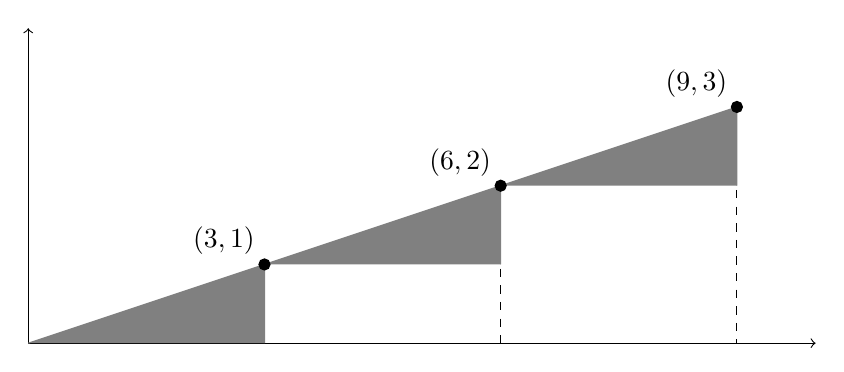
\begin{tikzpicture}[every node/.style={black}]
	\draw[->] (0,0)--(0,4);
	\draw[->] (0,0)--(10,0);

	\draw[dashed] (3,1)--(3,0);
	\draw[dashed] (6,2)--(6,0);
	\draw[dashed] (9,3)--(9,0);
	
	\filldraw[gray] (0,0)--(3,1)--(3,0);
	\filldraw[gray] (3,1)--(6,2)--(6,1);
	\filldraw[gray] (6,2)--(9,3)--(9,2);

	\filldraw (3,1) node[above left] {$(3,1)$} circle(2pt);
	\filldraw (6,2) node[above left] {$(6,2)$} circle(2pt);
	\filldraw (9,3) node[above left] {$(9,3)$} circle(2pt);
\end{tikzpicture}

Diagram for $(9,3)$ with $\gcd(9,3)=3$.
\end{center}

A sketch of a formal proof of this is the following:
\begin{enumerate}
\item There are a finite number of integer points in the square $(0,0)-(X,0)-(X,Y)-(0,Y)$,
a superset of the line between $(0,0)-(X,Y)$,
and all points of the line $(0,0)-(X,Y)$ can be uniquely ordered by their $X$ coordinate.
Hence there exits a unique integer point $(x,y)$ with minimal non-zero $X$ coordinate, this point may be $(X,Y)$ itself.
\item If a point $(x',y')$ is on the line then so is the point $(x'\mod x,y'\mod y)$.
Hence, by the minimality of $(x,y)$, all other integer points on the line are multiples of $(x,y)$ otherwise we could take $(x'\mod x,y'\mod y)$ as a smaller point.
\item Hence $x | X$, and let $d = \frac{X}{x}=\frac{Y}{y}$, then the set of integer points on the line $\{k(x,y)\,|\, k \in \{1,2,\cdots d\}\}$
\item By the minimality of $(x,y)$, $d$ must be the largest integer with the above property, meaning $d=\gcd(X,Y)$.
\end{enumerate}

But have you even considered how novel this answer is when the algebraic definition of $\gcd$ is used?
Let $(X,Y)\in\mathbb{N}^2_{>0}$ we can defined the $\gcd(X,Y)$ as:
\[\gcd(X,Y) = \min\{sX+rY\,|\,(s,r)\in\mathbb{Z}^2,\,sX+rY>0\}\]
And answer can be written as:
\begin{center}
\quad The number of solutions $(x,y)\in \mathbb{Z}^2$ to the equation $Xy-Yx=0$ such that $0<x\leq X$ is equal to $\min\{sX+rY\,|\,(s,r)\in\mathbb{Z}^2,\,sX+rY>0\}$.
\end{center}
